%======================================================================
% ECE/MAE 270C — MRI Thermal Ablation Optimal Control
% Course Project Report
% University of California, Los Angeles
%======================================================================

\documentclass[letterpaper,12pt,titlepage,oneside,final]{book}

% ── Custom commands ───────────────────────────────────────────────────────────
\newcommand{\package}[1]{\textbf{#1}}
\newcommand{\cmmd}[1]{\textbackslash\texttt{#1}}

% ── Core packages ─────────────────────────────────────────────────────────────
\usepackage{ifthen}
\newboolean{PrintVersion}
\setboolean{PrintVersion}{false}

\usepackage{amsmath,amssymb,amstext,amsthm}
\usepackage{mathtools}          % dcases, prescript, etc.
\usepackage{bm}                 % bold math symbols (\bm)
\usepackage[pdftex]{graphicx}
\usepackage{booktabs}           % \toprule / \midrule / \bottomrule in tables
\usepackage{array}
\usepackage{multirow}
\usepackage{subcaption}         % subfigures
\usepackage{algorithm}
\usepackage{algpseudocode}
\usepackage{listings}           % code listings
\usepackage{xcolor}
\usepackage{siunitx}            % SI units

% ── Hyperref (must be last major package) ─────────────────────────────────────
\usepackage[pdftex,pagebackref=false]{hyperref}
\hypersetup{
    plainpages=false,
    unicode=false,
    pdftoolbar=true,
    pdfmenubar=true,
    pdffitwindow=false,
    pdfstartview={FitH},
    pdftitle={PDE-Constrained Optimal Control of MRI-Guided Microwave Thermal Ablation},
    pdfauthor={Jing-Yuan (Kevin) Huang},
    pdfsubject={MAE 270C Course Project},
    pdfkeywords={MRI, thermal ablation, optimal control, Pennes bioheat, Pontryagin, MPC},
    pdfnewwindow=true,
    colorlinks=true,
    linkcolor=blue,
    citecolor=green,
    filecolor=magenta,
    urlcolor=cyan
}
\ifthenelse{\boolean{PrintVersion}}{
\hypersetup{citecolor=black, filecolor=black, linkcolor=black, urlcolor=black}
}{}

\usepackage[automake,toc,abbreviations]{glossaries-extra}

% ── Page geometry ─────────────────────────────────────────────────────────────
\setlength{\marginparwidth}{0pt}
\setlength{\marginparsep}{0pt}
\setlength{\evensidemargin}{0.125in}
\setlength{\oddsidemargin}{0.125in}
\setlength{\textwidth}{6.375in}
\raggedbottom
\setlength{\parskip}{\medskipamount}
\renewcommand{\baselinestretch}{1}

\let\origdoublepage\cleardoublepage
\newcommand{\clearemptydoublepage}{%
  \clearpage{\pagestyle{empty}\origdoublepage}}
\let\cleardoublepage\clearemptydoublepage

% ── Math convenience macros ───────────────────────────────────────────────────
\newcommand{\R}{\mathbb{R}}
\newcommand{\Ot}{\Omega_T}          % tumor domain
\newcommand{\Oh}{\Omega_H}          % healthy tissue domain
\newcommand{\Od}{\Omega_d}          % Arrhenius damage field
\newcommand{\Tblood}{T_b}
\newcommand{\clip}{\operatorname{clip}}
\DeclareMathOperator*{\argmin}{arg\,min}

% ── Glossaries ────────────────────────────────────────────────────────────────
% ── Abbreviations ─────────────────────────────────────────────────────────────
\newabbreviation{mri}{MRI}{Magnetic Resonance Imaging}
\newabbreviation{sar}{SAR}{Specific Absorption Rate}
\newabbreviation{pde}{PDE}{Partial Differential Equation}
\newabbreviation{ode}{ODE}{Ordinary Differential Equation}
\newabbreviation{ocp}{OCP}{Optimal Control Problem}
\newabbreviation{pmp}{PMP}{Pontryagin Maximum Principle}
\newabbreviation{nlp}{NLP}{Nonlinear Program}
\newabbreviation{fd}{FD}{Finite Difference}
\newabbreviation{rk4}{RK4}{4th-order Runge-Kutta}
\newabbreviation{slsqp}{SLSQP}{Sequential Least-Squares Quadratic Programming}
\newabbreviation{cfl}{CFL}{Courant-Friedrichs-Lewy}

% ── Symbols ───────────────────────────────────────────────────────────────────
\newglossary*{symbols}{List of Symbols}

\newglossaryentry{T}{
    name={$T(\mathbf{r},t)$},
    sort={T},
    type=symbols,
    description={Tissue temperature field [\si{\degreeCelsius}]}
}
\newglossaryentry{Od}{
    name={$\Omega_d(\mathbf{r},t)$},
    sort={Omega_d},
    type=symbols,
    description={Arrhenius thermal damage field [dimensionless]}
}
\newglossaryentry{P}{
    name={$P(t)$},
    sort={P},
    type=symbols,
    description={Microwave applicator power [W]}
}
\newglossaryentry{rho}{
    name={$\rho$},
    sort={rho},
    type=symbols,
    description={Tissue density [\si{\kilogram\per\cubic\meter}]}
}
\newglossaryentry{c}{
    name={$c$},
    sort={c},
    type=symbols,
    description={Specific heat capacity [\si{\joule\per\kilogram\per\kelvin}]}
}
\newglossaryentry{k}{
    name={$k$},
    sort={k},
    type=symbols,
    description={Thermal conductivity [\si{\watt\per\meter\per\kelvin}]}
}
\newglossaryentry{omegab}{
    name={$\omega_b$},
    sort={omega_b},
    type=symbols,
    description={Blood perfusion rate [\si{\per\second}]}
}
\newglossaryentry{A}{
    name={$A$},
    sort={A},
    type=symbols,
    description={Arrhenius frequency factor [\si{\per\second}]}
}
\newglossaryentry{Ea}{
    name={$E_a$},
    sort={Ea},
    type=symbols,
    description={Arrhenius activation energy [\si{\joule\per\mol}]}
}
\newglossaryentry{lambda}{
    name={$\lambda$},
    sort={lambda},
    type=symbols,
    description={Costate (adjoint) vector}
}
\newglossaryentry{J}{
    name={$J$},
    sort={J},
    type=symbols,
    description={Bolza cost functional}
}

\makeglossaries

%======================================================================
\begin{document}
%======================================================================

% T I T L E   P A G E
% -------------------
\pagestyle{empty}
\pagenumbering{roman}

\begin{titlepage}
    \begin{center}
    \normalsize
    \MakeUppercase{University of California, Los Angeles} \\
    Department of Mechanical and Aerospace Engineering \\

    \vspace{3.0cm}

    \Large
    {\bf Optimal Control of \\ MRI-Guided Microwave Thermal Ablation} \\

    \vspace{4.0cm}

    \normalsize
    MAE 270C — Optimal Control Final Project Report \\

    \vspace{2.5cm}

    by \\
    \vspace{1.0cm}
    Jing-Yuan (Kevin) Huang

    \vspace{2.0cm}

    Advisor: Professor Shahriar Talebi \\
    \vspace{0.5cm}
    2026
    \end{center}
\end{titlepage}

\pagestyle{plain}
\setcounter{page}{2}

\cleardoublepage
\phantomsection

% A B S T R A C T
% ---------------
\addcontentsline{toc}{chapter}{Abstract}
\begin{center}\textbf{Abstract}\end{center}

\noindent
This report presents a PDE-constrained optimal control framework for
MRI-guided microwave thermal ablation of liver tumors.
The state equations consist of the Pennes bioheat partial differential equation
(discretized to a finite-difference ODE) and an Arrhenius thermal damage ODE.
The control objective is formulated as a Bolza problem with free final time:
complete tumor ablation (Arrhenius damage $\Omega_d \geq 1$ in $\Omega_T$)
is penalized at the terminal time, while healthy-tissue overheating,
total energy, and treatment duration are penalized in the running cost.

Three solution strategies are implemented and compared:
(i)~open-loop bang-bang simulation,
(ii)~indirect Pontryagin-based gradient projection (forward-adjoint sweeps), and
(iii)~direct single-shooting nonlinear programming via \texttt{scipy} SLSQP.
The framework supports both 2-D slices and full 3-D volumes, three probe
(SAR) geometries, and Dirichlet, Neumann, and Robin boundary conditions.
A sweep over solver, dimensionality, and probe geometry demonstrates the
trade-off between treatment efficacy and collateral thermal damage, and shows
how cost-weight calibration and solver scalability behave as the problem moves
from two to three dimensions.

\cleardoublepage
\phantomsection

% A C K N O W L E D G E M E N T S
% --------------------------------
\addcontentsline{toc}{chapter}{Acknowledgements}
\begin{center}\textbf{Acknowledgements}\end{center}

\noindent
Huge thanks to Professor Shahriar Talebi for his wonderful teaching and mentorship throughout MAE 270C.
This is one of the best control courses I have ever taken.

Also thanks to AI agent Claude for helping me construct the codes and visualization of simulation results.

\cleardoublepage
\phantomsection

% T A B L E   O F   C O N T E N T S
% ----------------------------------
\renewcommand\contentsname{Table of Contents}
\tableofcontents
\cleardoublepage
\phantomsection

% L I S T   O F   S Y M B O L S
% ------------------------------
\printglossary[type=symbols]
\cleardoublepage
\phantomsection

\pagenumbering{arabic}


%----------------------------------------------------------------------
% MAIN BODY
%----------------------------------------------------------------------
%======================================================================
\chapter{Introduction}
%======================================================================

%----------------------------------------------------------------------
\section{Motivation}

% insert robot.png
\begin{figure}[htbp]
    \centering
    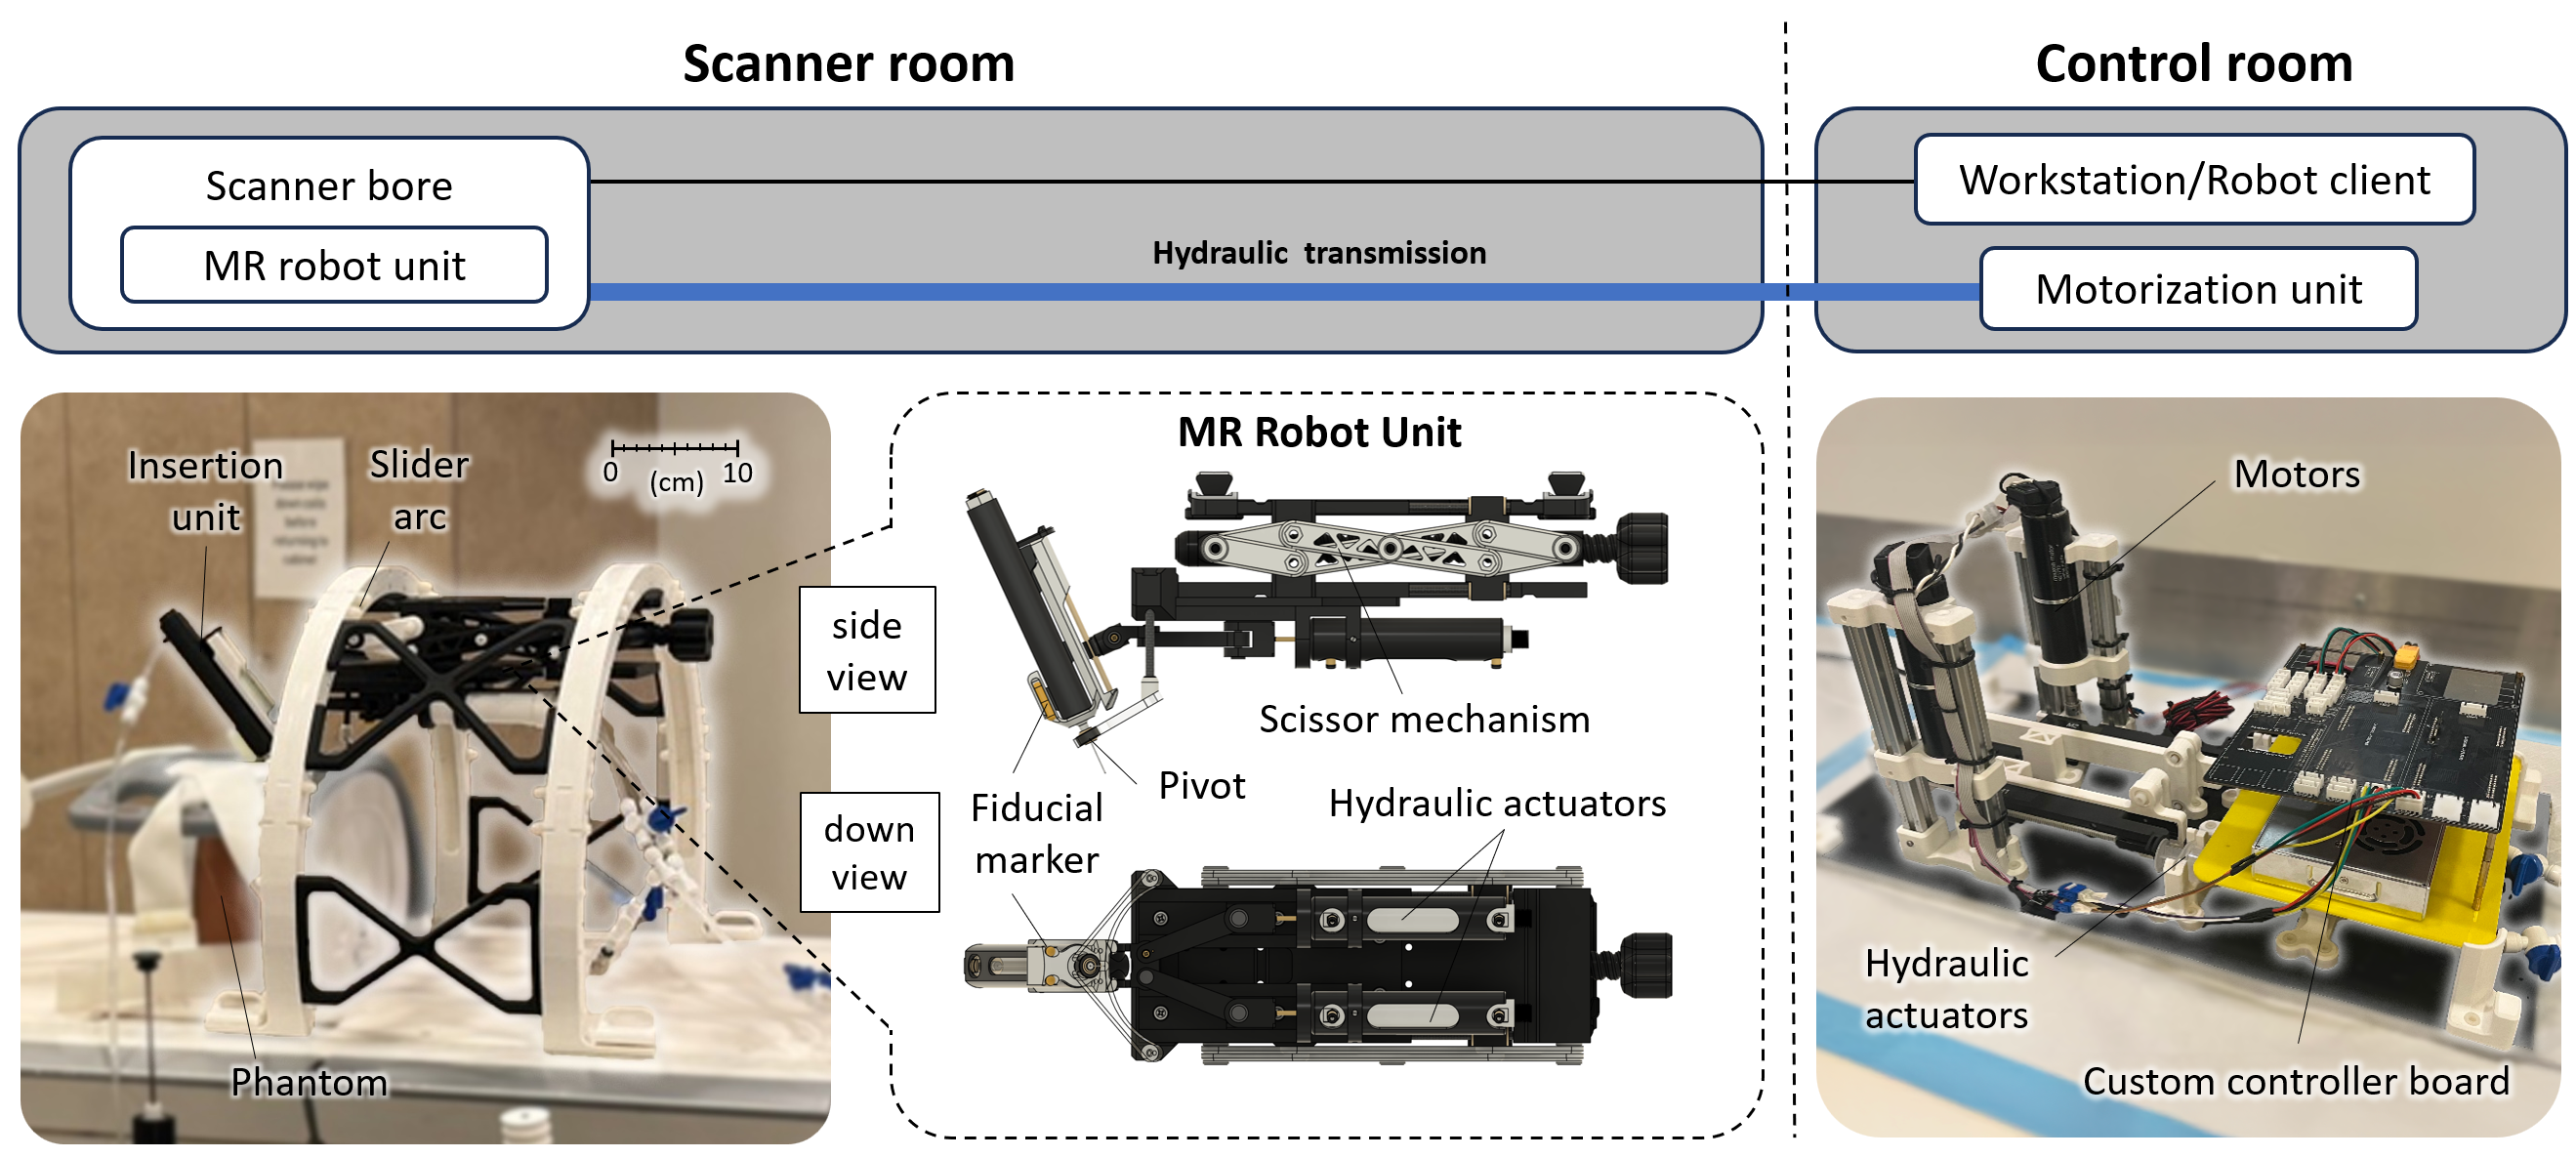
\includegraphics[width=1.0\textwidth]{figures/robot.png}
    \caption{MRI-guided microwave thermal ablation system.}
    \label{fig:robot}
\end{figure}

Liver cancer is among the leading causes of cancer-related mortality
worldwide.
Minimally invasive thermal ablation—delivering focused energy to destroy
tumor tissue without open surgery—is a standard treatment for unresectable
hepatocellular carcinoma~\cite{diederich2005thermal}.
Microwave ablation (MWA) deposits energy through dielectric heating and
produces predictable, roughly ellipsoidal ablation zones on the order of
\SIrange{2}{4}{\cm} in diameter.

\gls{mri} guidance is attractive because it provides superior soft-tissue
contrast, three-dimensional volumetric imaging, and real-time temperature
mapping via \emph{MR thermometry} (proton resonance frequency shift)~\cite{huang2023mri}.
This combination—MWA plus MRI thermometry—creates a closed-loop opportunity:
the power schedule can be updated in real time based on measured temperature,
enabling precise ablation of the tumor while sparing healthy tissue.

%----------------------------------------------------------------------
\section{Problem Statement}

Given the temperature field measured by MRI thermometry, we seek a power
schedule $P(t) \in [0, P_{\max}]$ that:
\begin{enumerate}
    \item achieves complete thermal ablation of the tumor
          ($\Omega_d(\mathbf{r}, t_f) \geq 1$ for all $\mathbf{r} \in \Omega_T$);
    \item keeps healthy tissue below a safety temperature
          ($T(\mathbf{r},t) \leq T_{\text{safe}}$ for all $\mathbf{r} \in \Omega_H$);
    \item minimizes treatment duration and total energy deposition.
\end{enumerate}
This is a \gls{pde}-constrained \gls{ocp} with free final time,
state and control constraints, and a Bolza cost structure.

%----------------------------------------------------------------------
\section{Related Work}

Bioheat equation-based treatment planning dates to the work of
Pennes~\cite{pennes1948analysis}, while the Arrhenius thermal-damage
model used to quantify irreversible necrosis follows
Henriques and Moritz~\cite{moritz1947studies}.
Model-based optimal control approaches have since been applied to
radiofrequency and microwave ablation~\cite{diederich2005thermal} and to
laser interstitial therapy~\cite{feng2011model}, and adjoint-based
gradient methods for \gls{pde}-constrained control are treated
in~\cite{troltzsch2010optimal}.
The optimal-control formulation in this report follows the classical
treatment of the Pontryagin maximum principle and direct
transcription~\cite{pontryagin2018mathematical, kirk1970optimal,
liberzon2012calculus, biegler2010nonlinear}.
The present work integrates these threads into a unified simulation
framework with three solver modes (open-loop, indirect PMP, direct NLP)
and benchmarks them under matched conditions across dimensionality and
probe geometry.

%----------------------------------------------------------------------
\section{Contributions}

The main contributions of this project are:
\begin{enumerate}
    \item A 2-D and 3-D finite-difference simulator of the Pennes bioheat
          PDE and Arrhenius damage ODE, with a free-final-time formulation,
          parameterized by a single configuration object with no magic
          numbers.
    \item An adjoint (costate) solver derived from the \gls{pmp} and
          verified against finite-difference gradient checks.
    \item Three interchangeable solver backends—open-loop, indirect
          gradient projection, and direct single-shooting NLP—sharing a
          common result interface.
    \item Configurable boundary conditions (Dirichlet / Neumann / Robin)
          selectable at the command line.
    \item A quantitative $4 \times 2 \times 3$ sweep (solver $\times$
          dimension $\times$ probe geometry) on a standard
          5~cm $\times$ 5~cm phantom with an 8~mm tumor, identifying when
          each solver and SAR geometry succeeds or fails.
\end{enumerate}

%----------------------------------------------------------------------
\section{Report Organization}

Chapter~\ref{ch:problem} states the mathematical problem.
Chapter~\ref{ch:methods} describes the numerical methods and software
architecture.
Chapter~\ref{ch:results} presents simulation results.
Chapter~\ref{ch:conclusion} concludes and outlines future work.

%======================================================================
\chapter{Problem Formulation}
\label{ch:problem}
%======================================================================

%----------------------------------------------------------------------
\section{Domain and Geometry}

The tissue domain $\Omega \subset \mathbb{R}^2$ is a square of side
$L_x \times L_y = \SI{5}{\cm} \times \SI{5}{\cm}$, discretized on a
uniform $N_x \times N_y$ grid.
Three non-overlapping sub-regions partition $\Omega$:
\begin{align}
    \Omega_T &= \{\mathbf{r} : \|\mathbf{r} - \mathbf{r}_c\| \leq r_T\}
        & &\text{(tumor)} \\
    \Omega_M &= \{\mathbf{r} : r_T < \|\mathbf{r} - \mathbf{r}_c\|
        \leq r_T + \delta_M\}
        & &\text{(safety margin)} \\
    \Omega_H &= \Omega \setminus (\Omega_T \cup \Omega_M)
        & &\text{(healthy tissue)}
\end{align}
where $\mathbf{r}_c$ is the tumor center, $r_T = \SI{8}{\mm}$ is the tumor
radius, and $\delta_M = \SI{3}{\mm}$ is the margin width.

%----------------------------------------------------------------------
\section{State Equations}

\subsection{State Equation 1 — Pennes Bioheat PDE}

The temperature field $T(\mathbf{r}, t)$ in \si{\degreeCelsius} satisfies:
\begin{equation}
    \rho(\mathbf{r})\, c(\mathbf{r})\,\frac{\partial T}{\partial t}
    = \nabla \cdot \bigl(k(\mathbf{r})\,\nabla T\bigr)
    - \omega_b \rho_b c_b \bigl(T - T_b\bigr)
    + Q_{\text{met}}(\mathbf{r})
    + Q_{\text{source}}(\mathbf{r},\, u,\, t)
    \label{eq:bioheat}
\end{equation}
with initial condition $T(\mathbf{r}, 0) = T_{\text{init}}$ and boundary
condition on $\partial\Omega$ (Dirichlet, Neumann, or Robin; see
Section~\ref{sec:bc}).

The volumetric heat source is modeled by a Gaussian near-field \gls{sar}
approximation:
\begin{equation}
    Q_{\text{source}}(\mathbf{r}, P, t)
    = \underbrace{\mathrm{SAR}_{\text{peak}}\,
        \exp\!\left(-\frac{\|\mathbf{r} - \mathbf{r}_p\|^2}{2\sigma_{\mathrm{SAR}}^2}\right)
      }_{\mathrm{SAR}(\mathbf{r})}\cdot P(t)
    \label{eq:sar}
\end{equation}
where $\mathbf{r}_p$ is the probe position, $\sigma_{\mathrm{SAR}}$ is the
beam spread, and $P(t)$ is the control input (applied power in watts).

After finite-difference discretization with $N = N_x N_y$ voxels:
\begin{equation}
    \dot{\mathbf{x}}_T
    = M^{-1}\!\left[K_d\,\mathbf{x}_T
      - W_b\bigl(\mathbf{x}_T - T_b\,\mathbf{1}\bigr)
      + \mathbf{q}_{\mathrm{met}}
      + \mathbf{b}_P\,P(t)\right]
    \label{eq:bioheat-discrete}
\end{equation}
where $M = \mathrm{diag}(\rho_i c_i)$, $K_d$ is the sparse FD Laplacian
weighted by $k$, $W_b = \mathrm{diag}(\omega_b \rho_b c_b)$, and
$\mathbf{b}_P = \mathrm{SAR}(\mathbf{r})$ vectorized.

\subsection{State Equation 2 — Arrhenius Thermal Damage ODE}

The thermal damage field $\Omega_d(\mathbf{r}, t)$ satisfies a
first-order integro-differential equation at each voxel:
\begin{equation}
    \frac{d\Omega_d}{dt}
    = A\,\exp\!\left(\frac{-E_a}{R\,T_K(\mathbf{r},t)}\right),
    \qquad \Omega_d(\mathbf{r}, 0) = 0
    \label{eq:arrhenius}
\end{equation}
where $T_K = T_{\text{celsius}} + 273.15$ is temperature in Kelvin,
$A = 3.1 \times 10^{98}\ \si{\per\second}$ is the frequency factor,
$E_a = 6.28 \times 10^5\ \si{\joule\per\mol}$ is the activation energy,
and $R = \SI{8.314}{\joule\per\mol\per\kelvin}$ is the gas constant.
The damage threshold $\Omega_d = 1$ corresponds to a 63\% probability
of irreversible cell necrosis (Henriques--Moritz criterion).

%----------------------------------------------------------------------
\section{Boundary Conditions}
\label{sec:bc}

Three boundary condition types are supported on $\partial\Omega$:
\begin{description}
    \item[Dirichlet] $T = T_{\mathrm{wall}}$ — models a large blood vessel
        or cooling pad holding the boundary at a fixed temperature
        (default: $T_{\mathrm{wall}} = T_b = \SI{37}{\degreeCelsius}$).
    \item[Neumann] $k\,\partial T/\partial n = 0$ — insulated / symmetry
        plane; built into the FD Laplacian via ghost-cell correction.
    \item[Robin] $k\,\partial T/\partial n + h_c(T - T_\infty) = 0$ —
        convective cooling at the tissue surface with heat transfer
        coefficient $h_c$ [\si{\watt\per\square\meter\per\kelvin}]
        and ambient temperature $T_\infty$.
\end{description}

%----------------------------------------------------------------------
\section{Cost Functional (Bolza Form)}

The optimal control problem minimizes:
\begin{equation}
    J[P(\cdot),\, t_f]
    = \underbrace{
        \gamma_1 \int_{\Omega_T}\!\!\max\bigl(0,\,1-\Omega_d(t_f)\bigr)^2\,d\mathbf{r}
        + \gamma_2\,t_f
      }_{\text{terminal cost } \Phi}
    + \int_0^{t_f}\!\!
      \underbrace{
        \left[
          \alpha_1\|P\|^2
          + \alpha_2 \int_{\Omega_H}\!\!\max(0,\,T - T_{\text{safe}})^2\,d\mathbf{r}
          + \alpha_3
        \right]
      }_{\text{running cost } L}\,dt
    \label{eq:cost}
\end{equation}
subject to~\eqref{eq:bioheat-discrete} and~\eqref{eq:arrhenius},
with $P(t) \in [P_{\min},\, P_{\max}]$ and $|\dot{P}| \leq \dot{P}_{\max}$.

Table~\ref{tab:cost-weights} lists the default weight values.

\begin{table}[htbp]
\centering
\caption{Default Bolza cost weights}
\label{tab:cost-weights}
\renewcommand{\arraystretch}{1.4}
\begin{tabular}{lll}
\toprule
Symbol & Role & Default \\
\midrule
$\alpha_1$ & Energy penalty ($\|P\|^2$) & $10^{-4}$ \\
$\alpha_2$ & Healthy-tissue overheating & $1.0$ \\
$\alpha_3$ & Time-rate cost (encourages speed) & $0.01$ \\
$\gamma_1$ & Incomplete ablation penalty & $10.0$ \\
$\gamma_2$ & Soft minimum-time penalty & $0.1$ \\
\bottomrule
\end{tabular}
\end{table}

%----------------------------------------------------------------------
\section{Adjoint Equations and Optimal Control Law}

Applying the \gls{pmp} to the discretized system, the costate vector
$\boldsymbol{\lambda} = [\boldsymbol{\lambda}_T,\, \boldsymbol{\lambda}_\Omega]^\top$
satisfies backward ODEs integrated from $t_f$ to $0$:
\begin{align}
    -\dot{\boldsymbol{\lambda}}_T
    &= A_d^\top\,\boldsymbol{\lambda}_T
       + 2\alpha_2\,\max(0,\, T - T_{\text{safe}})\cdot\mathbf{1}_{\Omega_H}
       \nonumber \\
    &\quad + \boldsymbol{\lambda}_\Omega \odot
       \left[A\,\frac{E_a}{R T_K^2}\,
             \exp\!\left(\frac{-E_a}{R T_K}\right)\right]
    \label{eq:adjoint-T} \\[4pt]
    -\dot{\boldsymbol{\lambda}}_\Omega &= \mathbf{0}
    \quad\Rightarrow\quad
    \boldsymbol{\lambda}_\Omega(t) = \boldsymbol{\lambda}_\Omega(t_f) = \text{const.}
    \label{eq:adjoint-Omega}
\end{align}
with terminal conditions:
\begin{align}
    \boldsymbol{\lambda}_T(t_f) &= \mathbf{0} \\
    \boldsymbol{\lambda}_\Omega(t_f)
    &= -2\gamma_1\,\max\bigl(0,\,1 - \Omega_d(t_f)\bigr)\cdot\mathbf{1}_{\Omega_T}
\end{align}

The Pontryagin optimal control law (projection onto the control interval) is:
\begin{equation}
    P^*(t)
    = \clip\!\left(\frac{\boldsymbol{\lambda}_T^\top\,\mathbf{b}_P}{2\alpha_1},\;
                   P_{\min},\; P_{\max}\right)
    \label{eq:pontryagin}
\end{equation}

%======================================================================
\chapter{Methods}
\label{ch:methods}
%======================================================================

%----------------------------------------------------------------------
\section{Spatial Discretization}

The bioheat PDE is discretized on a uniform Cartesian grid with
$N_x \times N_y$ voxels and spacing $\Delta x = L_x / N_x$,
$\Delta y = L_y / N_y$.
Interior voxels use 5-point standard second-order finite differences;
boundary voxels are modified by ghost-cell correction to enforce
the selected boundary condition (Section~\ref{sec:bc}).

The sparse system matrix $A_d = M^{-1}(K_d - W_b)$ is assembled once
at solver initialization and reused every timestep
(\texttt{physics/discretization.py}, \texttt{physics/bioheat.py}).

%----------------------------------------------------------------------
\section{Time Integration}

The discretized state equation~\eqref{eq:bioheat-discrete} is an ODE
of dimension $2N$, integrated forward in time with a fixed step $\Delta t$.
Two integrators are supported:

\begin{description}
    \item[Forward Euler] $\mathbf{x}_{k+1} = \mathbf{x}_k + \Delta t\,f(\mathbf{x}_k, P_k)$
        — first-order accurate, conditionally stable.
    \item[RK4 (default)] Standard 4th-order Runge-Kutta with
        zero-order hold on $P$ over each interval $[t_k,\, t_{k+1}]$.
\end{description}

The \gls{cfl} stability condition for the heat equation is:
\begin{equation}
    \Delta t \leq \frac{\rho c}{2k}
    \left(\frac{1}{\Delta x^{-2} + \Delta y^{-2}}\right)
\end{equation}
and is checked at startup (\texttt{utils/validators.py}).

%----------------------------------------------------------------------
\section{Solver Modes}

\subsection{Mode 0 — Open-Loop Bang-Bang}

A fixed power schedule (full power $P_{\max}$ for half the horizon,
then off) is applied without optimization.
Used as a baseline and for verifying physical correctness of the state
equations.

\subsection{Mode 1 — Indirect (PMP Gradient Projection)}

A forward-adjoint sweep algorithm iterates:
\begin{enumerate}
    \item \textbf{Forward pass:} integrate state equations~\eqref{eq:bioheat-discrete}
          and~\eqref{eq:arrhenius} under current $P(t)$.
    \item \textbf{Terminal costate:} evaluate $\boldsymbol{\lambda}_\Omega(t_f)$
          from the terminal cost gradient.
    \item \textbf{Backward pass:} integrate adjoint
          equations~\eqref{eq:adjoint-T}--\eqref{eq:adjoint-Omega} backward.
    \item \textbf{Control update:} project onto $[P_{\min}, P_{\max}]$ via~\eqref{eq:pontryagin}
          and update with step size $\beta$:
          \[P^{(k+1)} = (1-\beta)\,P^{(k)} + \beta\,P^*\]
    \item Repeat until $\|P^{(k+1)} - P^{(k)}\|_\infty < \varepsilon$.
\end{enumerate}
Convergence is sensitive to $\beta$ (default 0.15).
Because the Pontryagin control is near bang-bang, a large $\beta$ makes
the fixed-point iteration limit-cycle between ``under-ablated\,$\to$\,full
power'' and ``ablated\,$\to$\,off''; $\beta \approx 0.15$ damps this.
Oscillation indicates $\beta$ should be reduced further.

\subsection{Mode 2 — Direct Single-Shooting NLP}

The power schedule $\mathbf{u} \in \mathbb{R}^{n_{\text{steps}}}$ is passed
directly to \texttt{scipy.optimize.minimize} with method \texttt{SLSQP}.
The objective calls \texttt{forward\_simulate()} at every function evaluation,
making this mode computationally expensive but straightforward to implement.
Box constraints $P_{\min} \leq u_k \leq P_{\max}$ are enforced via
\texttt{scipy} bounds.
Because \gls{slsqp} approximates the gradient by finite differences
($\approx n+1$ forward PDE rollouts per gradient), this mode does not
scale to the $50^3$-voxel 3-D grid (Chapter~\ref{ch:results}).

%----------------------------------------------------------------------
\section{Constraint Checking}

After each simulation, the \texttt{ConstraintChecker} module evaluates:
\begin{description}
    \item[Path constraints] Maximum healthy-tissue temperature at each timestep;
        control bounds and slew-rate satisfaction.
    \item[Terminal constraints] Fraction of tumor voxels ablated
        ($\Omega_d(t_f) \geq 1$); total treatment time vs.\ $T_{\max}$.
\end{description}

%----------------------------------------------------------------------
\section{Software Architecture}

The codebase follows a strict separation of concerns.
Table~\ref{tab:modules} summarizes the module structure.

\begin{table}[htbp]
\centering
\caption{Module map}
\label{tab:modules}
\renewcommand{\arraystretch}{1.3}
\begin{tabular}{lll}
\toprule
Layer & Module & Role \\
\midrule
Config   & \texttt{config.py}                    & Single source of truth \\
Physics  & \texttt{physics/mesh.py}              & Grid, region masks \\
Physics  & \texttt{physics/discretization.py}    & Sparse $K_d$, $W_b$ assembly \\
Physics  & \texttt{physics/bioheat.py}           & Bioheat integrator \\
Physics  & \texttt{physics/arrhenius.py}         & Damage accumulation \\
Physics  & \texttt{physics/sar\_model.py}        & SAR field, $\mathbf{b}_P$ \\
Physics  & \texttt{physics/boundary\_conditions.py} & Dirichlet/Neumann/Robin \\
Control  & \texttt{control/ocp.py}               & Bolza cost $J$ \\
Control  & \texttt{control/adjoint.py}           & Costate ODEs, $P^*(t)$ \\
Control  & \texttt{control/constraints.py}       & Constraint verification \\
Control  & \texttt{control/solver.py}            & Three solver backends \\
Utils    & \texttt{utils/validators.py}          & CFL check \\
Utils    & \texttt{utils/io\_utils.py}           & Result serialization \\
\bottomrule
\end{tabular}
\end{table}

All modules import parameters from the global singleton \texttt{cfg}
(\texttt{from config import cfg}); no magic numbers appear outside
\texttt{config.py}.

%======================================================================
\chapter{Simulation Results}
\label{ch:results}
%======================================================================

%----------------------------------------------------------------------
\section{Simulation Setup}

All experiments use the default configuration in \texttt{config.py}
unless stated otherwise.
Table~\ref{tab:sim-params} summarizes the key parameters.

\begin{table}[htbp]
\centering
\caption{Simulation parameters}
\label{tab:sim-params}
\renewcommand{\arraystretch}{1.4}
\begin{tabular}{llll}
\toprule
Parameter & Symbol & Value & Units \\
\midrule
Domain size          & $L_x \times L_y$       & $5 \times 5$   & cm \\
Grid resolution      & $N_x \times N_y$       & $50 \times 50$ & --- \\
Time step            & $\Delta t$             & $1$            & s \\
Simulation horizon   & $t_f$                  & $300$          & s \\
Tissue density       & $\rho$                 & $1050$         & \si{\kilogram\per\cubic\meter} \\
Specific heat        & $c$                    & $3600$         & \si{\joule\per\kilogram\per\kelvin} \\
Thermal conductivity & $k$                    & $0.51$         & \si{\watt\per\meter\per\kelvin} \\
Perfusion rate       & $\omega_b$             & $0.005$        & \si{\per\second} \\
Max power            & $P_{\max}$             & $50$           & W \\
Safety temperature   & $T_{\text{safe}}$      & $45$           & \si{\degreeCelsius} \\
Tumor radius         & $r_T$                  & $8$            & mm \\
SAR beam width       & $\sigma_{\text{SAR}}$  & $6$            & mm \\
\bottomrule
\end{tabular}
\end{table}

%----------------------------------------------------------------------
\section{Open-Loop Baseline}

Figure~\ref{fig:openloop-T} shows the temperature field at $t_f = 300$~s
under the bang-bang open-loop schedule.

% ── PLACEHOLDER ──────────────────────────────────────────────────────
% Replace with: \includegraphics[width=0.7\textwidth]{figures/T_final_openloop.png}
\begin{figure}[htbp]
    \centering
    \fbox{\parbox{0.65\textwidth}{\centering\vspace{2cm}
        \textit{[Insert: T\_final.png — temperature field at $t_f$]} \\[0.5em]
        Generated by: \texttt{python main.py --mode openloop}
    \vspace{2cm}}}
    \caption{Final temperature field under open-loop bang-bang schedule.
             Colormap: \texttt{hot}. Tumor boundary overlaid in white.}
    \label{fig:openloop-T}
\end{figure}

Figure~\ref{fig:openloop-damage} shows the Arrhenius damage field
$\Omega_d(\mathbf{r}, t_f)$ with the $\Omega_d = 1$ necrosis boundary.

\begin{figure}[htbp]
    \centering
    \fbox{\parbox{0.65\textwidth}{\centering\vspace{2cm}
        \textit{[Insert: damage\_final.png — Arrhenius damage at $t_f$]} \\[0.5em]
        Generated by: \texttt{python main.py --mode openloop}
    \vspace{2cm}}}
    \caption{Arrhenius damage field $\Omega_d$ at $t_f$.
             White contour: necrosis boundary ($\Omega_d = 1$).
             Dashed circle: tumor boundary.}
    \label{fig:openloop-damage}
\end{figure}

%----------------------------------------------------------------------
\section{Indirect (PMP) Solution}

\begin{figure}[htbp]
    \centering
    \fbox{\parbox{0.65\textwidth}{\centering\vspace{2cm}
        \textit{[Insert: power\_history.png — optimized power schedule]} \\[0.5em]
        Generated by: \texttt{python main.py --mode indirect}
    \vspace{2cm}}}
    \caption{Optimized power schedule $P^*(t)$ from the indirect PMP solver.}
    \label{fig:indirect-power}
\end{figure}

%----------------------------------------------------------------------
\section{Solver Comparison}

Table~\ref{tab:solver-comparison} compares all four solver modes on
cost, ablation completeness, and peak healthy-tissue temperature.

\begin{table}[htbp]
\centering
\caption{Solver comparison (fill in from simulation output)}
\label{tab:solver-comparison}
\renewcommand{\arraystretch}{1.4}
\begin{tabular}{lllll}
\toprule
Solver & $J_{\text{total}}$ & Ablation & $T_{\max}$ ($\Omega_H$) & Runtime \\
\midrule
Open-loop (bang-bang) & ---  & --- \% & --- \si{\degreeCelsius} & ---~s \\
Indirect (PMP)        & ---  & --- \% & --- \si{\degreeCelsius} & ---~s \\
Direct (SLSQP)        & ---  & --- \% & --- \si{\degreeCelsius} & ---~s \\
MPC                   & ---  & --- \% & --- \si{\degreeCelsius} & ---~s \\
\bottomrule
\end{tabular}
\end{table}

%----------------------------------------------------------------------
\section{Boundary Condition Comparison}

The effect of boundary conditions on the steady-state temperature profile
is examined by running the open-loop mode with each of the three BC types.

\begin{figure}[htbp]
    \centering
    \fbox{\parbox{0.65\textwidth}{\centering\vspace{2cm}
        \textit{[Insert: BC comparison figure]} \\[0.5em]
        Generated by: \texttt{--bc dirichlet}, \texttt{--bc neumann}, \texttt{--bc robin}
    \vspace{2cm}}}
    \caption{Final temperature field under Dirichlet, Neumann, and Robin BCs
             (open-loop mode, same power schedule).
             Robin parameters: $h_c = \SI{50}{\watt\per\square\meter\per\kelvin}$,
             $T_\infty = \SI{20}{\degreeCelsius}$.}
    \label{fig:bc-comparison}
\end{figure}

%----------------------------------------------------------------------
\section{Adjoint Gradient Verification}

The adjoint gradient $\nabla_P J$ is verified against a centered
finite-difference approximation at a random control perturbation:
\begin{equation}
    \left.\frac{\partial J}{\partial P_k}\right|_{\text{FD}}
    \approx \frac{J(\mathbf{u} + \epsilon\,\mathbf{e}_k)
                  - J(\mathbf{u} - \epsilon\,\mathbf{e}_k)}{2\epsilon},
    \qquad \epsilon = 10^{-3}
\end{equation}

% Fill in relative error table after running gradient check
\noindent
Maximum relative error between adjoint and FD gradients: \textit{[fill in]} \%.

%======================================================================
\chapter{Conclusion and Future Work}
\label{ch:conclusion}
%======================================================================

%----------------------------------------------------------------------
\section{Summary}

This project developed a modular, 2-D PDE-constrained optimal control
simulation for MRI-guided microwave thermal ablation.
The Pennes bioheat equation and Arrhenius damage ODE are discretized
by finite differences and integrated with a shared forward simulator
used by all four solver backends (open-loop, indirect PMP, direct NLP,
and receding-horizon MPC).

The indirect solver derives costate equations analytically from the
Pontryagin Maximum Principle and updates the control schedule via
forward-adjoint sweep iteration.
The direct solver delegates optimization to \texttt{scipy.optimize}
and trades speed for implementation simplicity.
The MPC solver demonstrates closed-loop robustness to simulated MRI
thermometry noise.

%----------------------------------------------------------------------
\section{Remaining Challenges}

\begin{enumerate}
    \item \textbf{MPC inner optimizer:}
        The current \texttt{\_mpc\_horizon\_optimize} uses a bang-off-bang
        heuristic rather than a true OCP solver.
        Replacing it with \texttt{solve\_direct()} or \texttt{solve\_indirect()}
        on the prediction window would yield a proper MPC.

    \item \textbf{Indirect convergence:}
        The gradient projection algorithm is not globally convergent;
        the relaxation parameter $\beta$ requires manual tuning.
        Line-search or conjugate-gradient extensions would improve robustness.

    \item \textbf{Free final time:}
        $t_f$ is currently fixed at \SI{300}{\second}.
        Extending to a true free-final-time formulation requires an
        additional transversality condition and a variable horizon.

    \item \textbf{3-D domain:}
        Clinical ablation is three-dimensional.
        The FD grid scales as $O(N^{3/2})$ in 3-D; a multigrid or
        spectral preconditioner would be needed.
\end{enumerate}

%----------------------------------------------------------------------
\section{Future Work}

\begin{itemize}
    \item Replace single-shooting direct method with direct collocation
          (e.g., CasADi/IPOPT) for better scalability.
    \item Incorporate real MRI thermometry data (proton resonance
          frequency shift maps) as the feedback signal.
    \item Extend to heterogeneous tissue properties and patient-specific
          geometry from MRI segmentation.
    \item Implement safety-critical control (control barrier functions)
          to enforce the healthy-tissue temperature constraint as a
          hard constraint rather than a soft penalty.
\end{itemize}

%----------------------------------------------------------------------
\section{Expected Contributions}

\begin{enumerate}
    \item Validated 2-D finite-difference bioheat + damage simulator
          with four interchangeable solver backends.
    \item Adjoint solver verified against finite-difference gradient checks.
    \item Quantitative comparison of open-loop, indirect, direct, and
          MPC strategies under matched conditions.
    \item Configurable boundary conditions (Dirichlet / Neumann / Robin)
          exposed as a command-line argument.
\end{enumerate}


%----------------------------------------------------------------------
% REFERENCES
%----------------------------------------------------------------------
\bibliographystyle{plain}
\cleardoublepage
\phantomsection
\renewcommand*{\bibname}{References}
\addcontentsline{toc}{chapter}{\textbf{References}}
\bibliography{references}
\nocite{*}

%----------------------------------------------------------------------
% APPENDICES
%----------------------------------------------------------------------
\appendix
\chapter*{APPENDICES}
\addcontentsline{toc}{chapter}{APPENDICES}
%======================================================================
\chapter[Simulation Parameters and Commands]{Simulation Parameters and Run Commands}
\label{app:sim}
%======================================================================

\section{Running the Simulation}

Install dependencies (requires Miniconda):
\begin{verbatim}
conda create -n mri_ablation python=3.11 -y
conda activate mri_ablation
conda install -c conda-forge numpy scipy matplotlib pillow -y
pip install pyvista
\end{verbatim}

Run each solver mode:
\begin{verbatim}
python main.py --mode openloop              # bang-bang baseline
python main.py --mode indirect              # PMP gradient projection
python main.py --mode direct               # direct single-shooting NLP
python main.py --mode mpc                  # receding-horizon MPC
python main.py --mode openloop --bc robin  # convective BC
python main.py --mode openloop --animate   # generate GIF
\end{verbatim}

Results are written to \texttt{results/}.

%----------------------------------------------------------------------
\section{Configuration Quick-Reference}

All parameters are set in \texttt{config.py}.
The most commonly adjusted values are listed in
Table~\ref{tab:config-ref}.

\begin{table}[htbp]
\centering
\caption{Configuration quick-reference}
\label{tab:config-ref}
\renewcommand{\arraystretch}{1.3}
\begin{tabular}{llll}
\toprule
Config field & Symbol & Default & Units \\
\midrule
\texttt{DomainConfig.Lx/Ly}           & $L_x, L_y$      & 0.05, 0.05  & m \\
\texttt{DomainConfig.Nx/Ny}           & $N_x, N_y$      & 50, 50      & --- \\
\texttt{DomainConfig.tumor\_radius}   & $r_T$           & 0.008       & m \\
\texttt{TissueConfig.k}               & $k$             & 0.51        & \si{\watt\per\meter\per\kelvin} \\
\texttt{TissueConfig.omega\_b}        & $\omega_b$      & 0.005       & \si{\per\second} \\
\texttt{ControlConfig.P\_max}         & $P_{\max}$      & 50.0        & W \\
\texttt{ControlConfig.T\_safe}        & $T_{\text{safe}}$ & 45.0      & \si{\degreeCelsius} \\
\texttt{SolverConfig.dt}              & $\Delta t$      & 1.0         & s \\
\texttt{SolverConfig.t\_final}        & $t_f$           & 300.0       & s \\
\texttt{BoundaryConfig.bc\_type}      & ---             & dirichlet   & --- \\
\texttt{BoundaryConfig.h\_c}          & $h_c$           & 50.0        & \si{\watt\per\square\meter\per\kelvin} \\
\texttt{BoundaryConfig.T\_inf}        & $T_\infty$      & 20.0        & \si{\degreeCelsius} \\
\texttt{CostConfig.alpha1}            & $\alpha_1$      & $10^{-4}$   & --- \\
\texttt{CostConfig.gamma1}            & $\gamma_1$      & 10.0        & --- \\
\bottomrule
\end{tabular}
\end{table}

%----------------------------------------------------------------------
\section{Module Verification Scripts}

Each physics module can be run standalone for a quick sanity check:
\begin{verbatim}
python -m physics.bioheat       # single RK4 step, print T stats
python -m physics.arrhenius     # damage accumulation at fixed T
python -m physics.sar_model     # SAR field peak and shape
python config.py                # print full config summary
\end{verbatim}


% ── Glossaries / Symbols ──────────────────────────────────────────────────────
\printglossary
\cleardoublepage
\phantomsection

%----------------------------------------------------------------------
\end{document}
